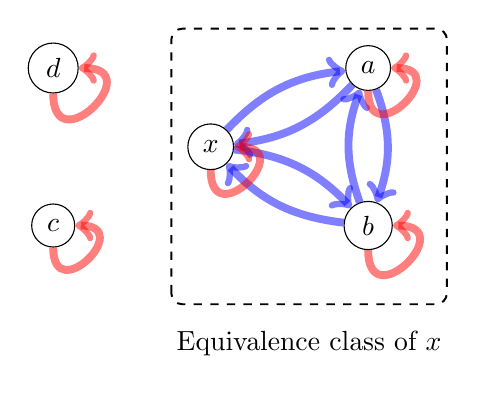
\begin{tikzpicture}
	\tikzset{
		main node/.style={circle, draw, fill=blue!20, minimum size=1cm, font=\sffamily},
		class node/.style={ellipse, draw, thick, red, minimum height=2.5cm, minimum width=4cm, align=center},
		path/.style={->, thick, shorten <=2pt, shorten >=2pt},
		reflexive/.style={->, line width=1mm, loop, looseness=5, in=0, out=-90, red, opacity=.5},
		symmetric/.style={->, line width=1mm, blue, bend left=20, opacity=.5},
		transitive/.style={->, line width=1mm, green!75!black, bend left=50pt, opacity=.5},
		label distance=3mm
	}
	% Elements of S
	\node (x) at (0,0) [circle, draw] {$x$};
	\node (a) at (2,1) [circle, draw] {$a$};
	\node (b) at (2,-1) [circle, draw] {$b$};
	\node (c) at (-2,1) [circle, draw] {$d$};
	\node (d) at (-2,-1) [circle, draw] {$c$};
	
	\foreach \x/\y in {x/a, a/b, x/b} {
		\draw[symmetric] (\x) to (\y);
		\draw[symmetric] (\y) to (\x);
	}
	
	\foreach \x in {x,a,b,c,d} {
		\draw[reflexive] (\x) to (\x);
	}
	% Draw equivalence class
	\draw[rounded corners, dashed, line width=.25mm] (-.5,-2) rectangle (3,1.5);
	\node at (1.25,-2.5) {Equivalence class of $x$};
	
	% Connect x with equivalent elements
%	\draw (x) -- (a);
%	\draw (x) -- (b);
\end{tikzpicture}
